\chapter{Background}
\label{background}

\section{RoboCup Competition}

The RoboCup Competition, in its short history, has grown to a well-established annual event bringing together the best robotics researchers from all over the world. The initial conception by Hiroaki Kitano~\cite{robocup} in 1993 led to the formation of the RoboCup Federation with a bold vision: ``By the year 2050, to develop a team of fully autonomous humanoid robots that can win against the human world soccer champions''.The uniqueness of RoboCup stems from the real-world challenge it poses, whereby the core problems of robotics (perception, cognition, action, coordination) must be addressed simultaneously under real-time constraints. The proposed solutions are tested on a common benchmark environment through soccer games in various leagues,with the goal of promoting the best approaches, and ultimately advancing the state-of-the-art in the area. 

\section{RoboCup Leagues}

Beyond soccer, RoboCup now includes also competitions in search-and-rescue missions (RoboRescue), home-keeping tasks (RoboCup@Home), robotic performances (RoboDance), and simplified soccer leagues for K-12 students (RoboCup Junior). Broadening the research areas where RoboCup focuses, was a very interesting and clever addition, which enables all the more scientists and researchers combine their expertise in order to solve real world problems. A lot of progress has been made so far in many disciplines of robotics and RoboCup has been established in one of the most important events around the world.

\section{RoboRescue}

RoboRescue initiated from the need of people to create robots capable of operating in hostile or inaccessible environments by humans. This area is very motivating in terms of helping the humanity while promoting robotics. Multi-agent team work coordination, physical robotic agents and rescue strategies are all being tested in real or simulated environments (Figure~\ref{fig:roboRescue}), using sensors including cameras, temperature sensors, $CO_2$ sensors and other that allow for fast and efficient human body localization.

\begin{figure}[h]
	\begin{center}
		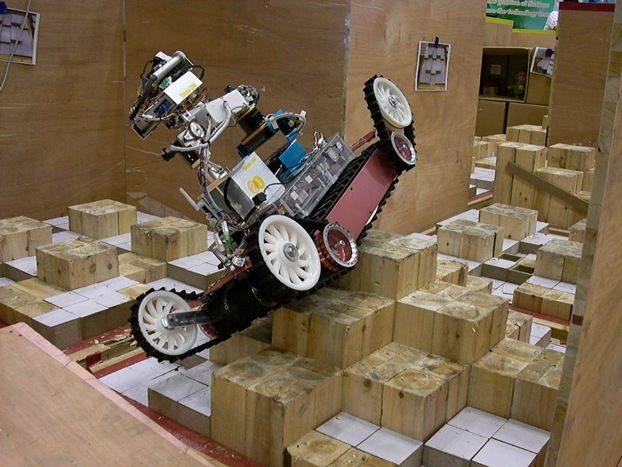
\includegraphics[height = 6cm]{Chapter1/figures/roboRescue.jpeg}
 		\caption{RoboRescue environments can become extremely hostile for robots.}
 		\label{fig:roboRescue}
	\end{center}
\end{figure}

\section{RoboCup@Home}

The RoboCup@Home league aims to develop service and assistive robot technology with high relevance for future personal domestic applications. It is the largest international annual competition for autonomous service robots and is part of the RoboCup initiative. A set of benchmark tests is used to evaluate the robots' abilities and performance in a realistic non-standardized home environment setting (Figure~\ref{fig:robocup@home}).

Most of the research lies in many domains including Human-Robot-Interaction and Cooperation, Navigation and Mapping in dynamic environments, Computer Vision and Object Recognition under natural light conditions, Object Manipulation, Adaptive Behaviors, Behavior Integration, Ambient Intelligence, Standardization and System Integration.

\begin{figure}[h]
	\begin{center}
		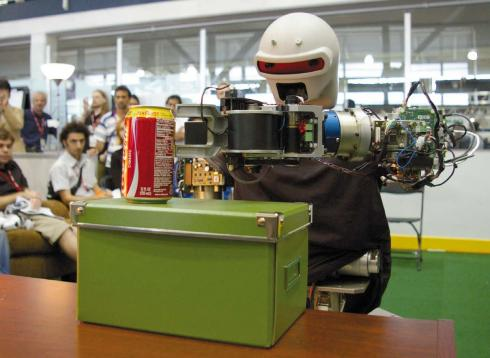
\includegraphics[height = 6cm]{Chapter1/figures/robocup@home.jpeg}
 		\caption{Robocup@Home represents a social aspect of robotics interacting with people.}
 		\label{fig:robocup@home}
	\end{center}
\end{figure}


\section{RoboCup Junior}

Robocup Junior is one of the smaller and less competitive, in terms of antagonism sub-domain of RoboCup, which is mainly intended in the preparation of gifted children interested in robotics. It is very important to understand that this competition has nothing to be jealous of the other leagues, but in fact share the same vision and the required dedication to excel.

\subsection{Dance}

RoboDance might one say to be the most amusing competition of RoboCup, where robots are performing in front of their audience. Dances, most of times, are innovative and unique. Developers are being judged on the novelty of motions, the cooperation of the robots, and finally the synchronization of the robot motion according to the music.

\subsection{Rescue}

Rescue in the Junior league, is a simplified version of RoboRescue and is limited in the line-following problem. Each team has to qualify from a number of tracks whose difficulty gradually increases. The trials are judged on the duration of the track completion and on the agent's behavior in misleading parts of the track, such as line intersections, or line gaps.

\subsection{Soccer}

The soccer competition is played by two cylindrical robots which share the same features and play soccer in a box or in a table surrounded by low walls. This is by far the most exciting competition in Robocup Junior and the most demanding.


\section{RoboCup Soccer League}

The RoboCup Soccer League, is the domain with the most fans. In this league researchers combine their technical knowledge in order to prepare the best robotic soccer team among other universities.

\subsection{The Standard Platform League}

Standard Platform League (SPL) of the RoboCup competition is the most popular league, featuring two to four humanoid Aldebaran Nao robot players in each team. This league was formerly known as the Four-Legged League with Sony Aibo robots, which were replaced in 2008 by Aldebaran Nao (Figure~\ref{fig:spl}). Games take place in a $4 m \times 6 m$ field marked with thick white lines on a green carpet. The two colored goals (sky-blue and yellow) also serve as landmarks for localizing the robots in the field. Each game consists of two 10-minute halves and teams switch colors and sides at halftime. There are several rules enforced by human referees during the game. For example, a player is punished with a 30-seconds removal from the field if he performs an illegal action, such as pushing an opponent for more than three seconds, grabbing the ball between his legs for more than three seconds, or entering his own goal area as a defender.

\begin{figure}[h]
	\begin{center}
		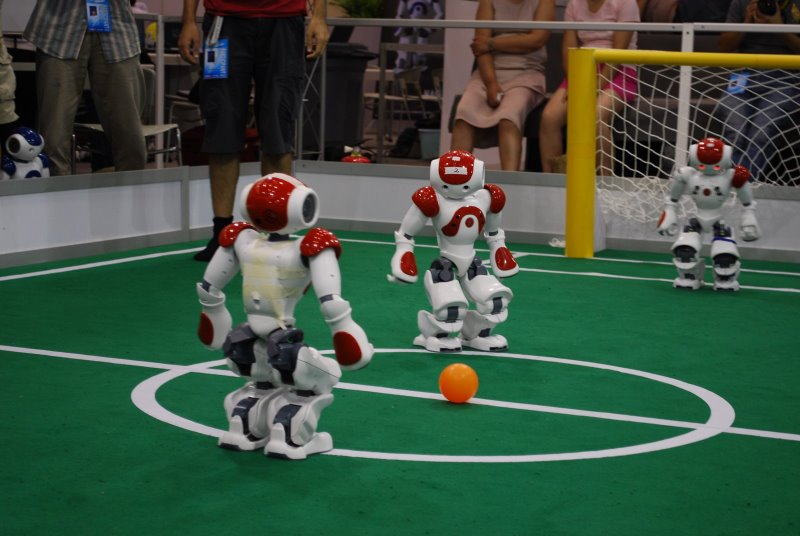
\includegraphics[height = 8cm]{Chapter1/figures/spl.jpg}
 		%\caption{Middle size league teams preparing before a game in RoboCup German Open 2007.}
		\caption{Standard Platform League game in Robocup 2008( Opponents should be in different colors, but there was a lack of Nao robots in that event due to malfunctions )}
 		\label{fig:spl}
	\end{center}
\end{figure}


The main characteristic of the Standard Platform League is that no hardware changes are allowed; all teams use the exact same robotic platform and differ only in terms of their software. This convention results to the league's enrichment of a unique set of features: autonomous player operation, vision-based perception, legged locomotion and action. Given that the underlying robotic hardware is common for all competing teams, research effort has been focused on the development of more efficient algorithms and techniques for visual perception, active localization, omni-directional motion, skill learning, and coordination strategies. During the course of the years, one could easily notice a clear progress in all research directions.

\subsection{Simulation League}

Every year there is a number of simulation games taking place in RoboCup competitions. These include 2D soccer games, where teams consist of 11 agents providing to developers with a perfect multi-agent environment to tune and benchmark their solutions. 3D simulation games exist as well; usage of physics engines demand more realistic approaches.

Simulators offer the ability to control the amount of ``negative'' realism added in these environments; thus, it is a great way to allow researchers work focusing in multi-agent cooperation approaches and other state-of-the-art algorithms, abstracting from real-world problems (gravity, forces etc).

In RoboCup 2008, three of the most important simulation leagues, were the official RoboCup Simulation League run in an open source simulator, the Microsoft Robotics Studio competition, and the Webots RoboStadium.

\subsection{Small Size League}

A Small Size robot soccer game takes place between two teams of five robots each. Each robot must fit within an 180mm diameter circle and must be no higher than 15cm, unless they use on-board vision. Robots play soccer on a 6.05m long by 4.05m wide, green carpeted field with an orange golf ball. Vision information is either processed on-board the robot or is transmitted back to the off-field PC. Another off-field PC is being used to communicate referee commands and position information to the robots, when an extra camera mounted on top of the field serves as the vision sensor. Typically, off-field PCs are used in the coordination and control of the robots. Communication is wireless and typically use dedicated commercial FM transmitter/receiver units\footnote{http://small-size.informatik.uni-bremen.de/rules:main}.

\subsection{Middle Size League}

Middle Size is more competitive and demanding, having the largest field dimensions among other leagues (Figure~\ref{fig:middleSize}). Two teams of mid-sized robots consist of 5 players each, with all sensors on-board play soccer on a field of $18 m \times 12 m$, whereas relevant objects are distinguished by colors only. Communication among robots (if any) is supported on wireless communications. Once again, no external intervention by humans is allowed, except to insert or remove robots in/from the field. These robots are the best players far among other leagues. The robots' bodies are heavy enough having powerful motors, heavy batteries, omni-directional camera, and a full laptop computer running in every robot; characteristics that make this league a great domain for research.


\begin{figure}[h]
	\begin{center}
		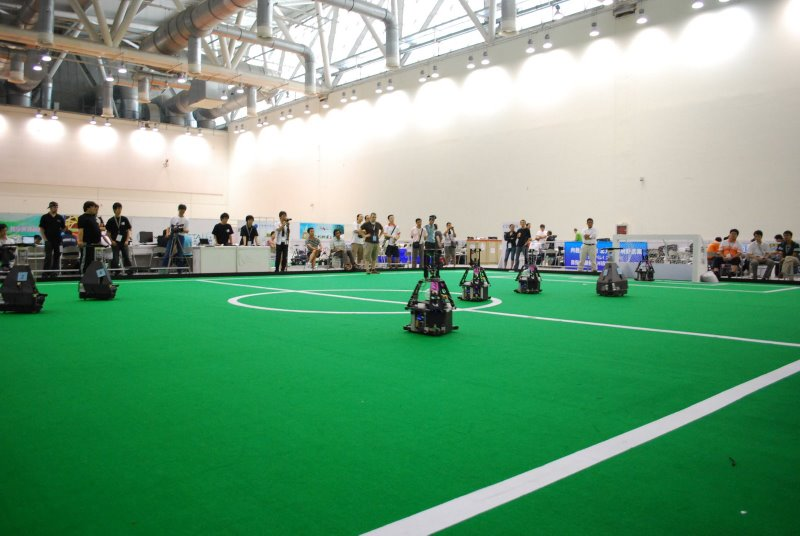
\includegraphics[height = 8cm]{Chapter1/figures/middleSize1.jpg}
 		%\caption{Middle size league teams preparing before a game in RoboCup German Open 2007.}
		\caption{Middle size league game in Robocup 2008.}
 		\label{fig:middleSize}
	\end{center}
\end{figure}

\subsection{Humanoid League}

The Humanoid League is one of the most dynamically progressing leagues and the one closest to the 2050's goal. In this league, autonomous robots with a human-like body plan and human-like senses play soccer against each other. In addition to soccer competitions, technical challenges take place. The robots are divided into two size classes: KidSize (30-60cm height) and TeenSize (100-160cm height). Dynamic walking, running, and kicking the ball while maintaining balance, visual perception of the ball, other players, and the field, self-localization, and team play are among the many research issues investigated in this league. Several of the best autonomous humanoid robots in the world compete in the RoboCup Humanoid League\footnote{http://www.tzi.de/humanoid/bin/view/Website/WebHome}.

\section{Kouretes Team}

{\em Kouretes} Team, is a collaboration of the Intelligent Systems Laboratory at the Department of Electronic and Computer Engineering, and the Intelligent Systems and Robotics Laboratory at the Department of Production Engineering and Management. It was the first Greek team participating in Robocup competitions, specializing in the Standard Platform League and the MSRS Simulation League. The team's name, {\em Kouretes}, comes from the Ancient Greek Mythology. Formerly consisted by four AIBO robots named Epimedes, Paionaios, Iasios, and Idas, after the five Kouretes brothers, who were ancient Cretan warriors.The fifth brother, Hercules, represents all the human members of the team. Since Spring 2008 four NAO robots joined the team, but they have not been named yet.

{\em Kouretes} have participated in many competitions, exhibitions, and affairs, but the highlights of the steep orbit the team followed were the second place in Robocup 2007, Atlanta, USA in the MSRS Simulation League and the first and third place in Robocup 2008, Suzhou, China in the MSRS Simulation League, and the Standard Platform League accordingly. 
%
%{\em Kouretes} team's 2008 formation in Figure~\ref{fig:kouretes2008formation} from left to right in the front row are Andreas Panakos (SPL), Daisy Chroni (Simulation Team), Alexandros Paraschos (SPL), Stathis Vafias (Simulation Team), and in the back row Professor Michail G. Lagoudakis (Kouretes Team Leader) and Georgios F. Pierris (SPL). Lastly but not least, we must mention the other two members of {\em Kouretes} supporting the team from our base, Lefteris Chatzilaris(Simulation Team Robostadium), and Evangelos Vazaios(SPL), who entered the team back in 2008, working now actively and full time, looking forward to Robocup 2010 competition in Singapore, Singapore.

\begin{figure}[h]
	\begin{center}
		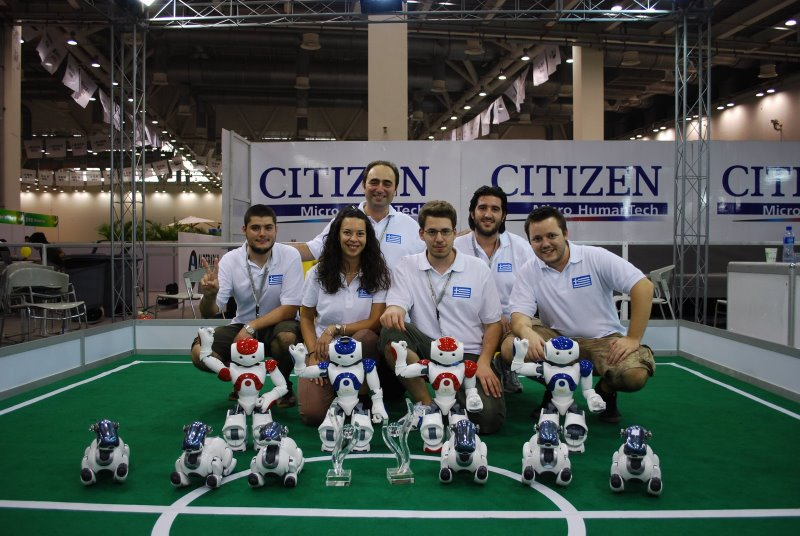
\includegraphics[height = 9cm]{Chapter1/figures/kouretesTeam2008formation.jpg}
		\caption{\small{Kouretes team 2008 formation. From left to right in the front row are Andreas Panakos(SPL), Daisy Chroni(Simulation Team), Alexandros Paraschos(SPL), Stathis Vafias(Simulation Team), and in the back row Professor Michail G. Lagoudakis( Kouretes Team Leader ) and Georgios F. Pierris(SPL).}}
 		\label{fig:kouretes2008formation}
	\end{center}
\end{figure}

More information and news of the team but also its members can be found at \url{http://www.kouretes.gr}.

\section{NAO Robot}

Nao, in its final version, is a 58 cm, 4.3 Kg humanoid robot. To this time, Nao has not been released commercially yet, however Aldebaran's goal is to eventually promote Nao as an educational robotic platform and a family entertainment robot affordable to most budgets. The initial limited edition of the robot (RoboCup edition v2) made its debut at RoboCup 2008. The Nao robot carries a full computer on board with an x86 AMD Geode processor at 500 MHz, 256 MB SDRAM, and 1 GB flash memory running an Embedded Linux distribution. It is powered by a 6-cell Lithium-Ion battery which provides about 45 minutes of continuous operation and communicates with remote computers via an IEEE 802.11g wireless or a wired ethernet link. The Nao robot features a variety of sensors and actuators.

\subsection{Cameras}

In the NAO V2 robot, only one camera was mounted in the head. It was a 30fps, $640 \times 480$ color camera, provided with a rich API, allowing us many interventions, in order to get the best result, under any reasonable lighting conditions. Unfortunately, probably a driver bug caused us a lot of problems, since the camera output was in bytes in YUV422 format. The ordering was of U, Y1, V, Y2, however sometimes a shift in this order flipped the U and V in the resulting image. Even though, most colors were unaffected, orange was light purple in the output. Some solutions to this problem have been suggested by GT/CMU, rUNSWift and other, but this problem finally solved in the V3 robot by Aldebaran.

\begin{figure}
	\begin{center}
		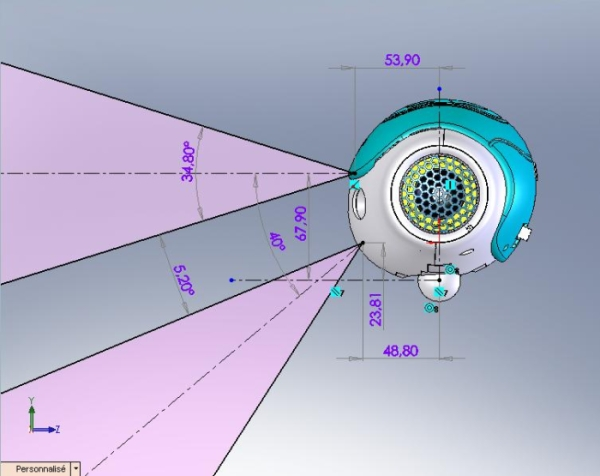
\includegraphics[height=6cm]{Chapter1/figures/fieldOfView.jpg}
		\caption{Nao's field of View}
		\label{fig:fieldOfView}
	\end{center}
\end{figure}

During the first games, it was clear that NAO did not have a clear view in the short frontal area. Even when the Head Pitch Joint angle was at its lowest value, the ball was not visible and its position was not determinable according to the NAO's legs. Thus, most teams were obliged to create a bend motion, not only consuming gameplay time, but also stressing the NAO's joints. The answer from Aldebaran, was to mount a second identical camera in the head, pointing directly in the short frontal area. In the NAO V3, these cameras are mounted on the head in vertical alignment providing non-overlapping views of the lower and distant frontal areas (Figure ~\ref{fig:fieldOfView}), but only one is active each time and the view can be switched from one to the other almost instantaneously.


\subsection{Connectivity}

Connecting to a robot is a major concept, thus Aldebaran provide us three means of connection. The NAO robot, can be connected directly or sharing the same network, through a wired ethernet link. Additionally, an IEEE 802.11g wireless card is available, which is the frequent way of connection, due to the lack of forces applied to the robot through the network cable, and finally Aldebaran provides a serial cable, which comes into play when we want to debug the robot, and read messsages concerning the Nao's procedures.


\subsection{Audio, Sensors, Various}

A pair of microphones allows for stereo audio perception. Two ultrasound sensors on the chest allow Nao to sense obstacles in front of it and a rich inertial unit (a 2-axis gyroscope and a 3-axis accelerometer) in the torso provides real-time information about its instantaneous body movements. Finally, an array of force sensitive resistors on each foot delivers feedback on the forces aplied to the feet, while encoders on all servos record the actual joint position at each time and two bumpers on the feet provide information on collisions of the feet with obstacles. The Nao robot has a total of 21 degrees of freedom; 4 in each arm, 5 in each leg, 2 in the head, and 1 in the pelvis (there are 2 pelvis joints which are coupled together on one servo and cannot move independently). Stereo loudspeakers and a series of LEDs complement its motion capabilities with auditory and visual actions.

\subsection{NaoQi}

The Nao programming environment is based on the proprietary NaoQi framework which serves as a middleware between the robot and high-level languages, such as C, C++, and Python. NaoQi offers a distributed programming and debugging environment which can run embedded on the robot or remotely on a computer offering an abstraction for event-based, parallel and sequential execution. Its architecture is based on modules and brokers which can be executed onboard the robot or remotely and allows the seamless integration of various heterogeneous components, including proprietary and custom-made functionality.

\section{General Overview}

In overall, Aldebaran Robotics designed and assembled a low-cost robot, which can be a great, not only scientific, but also entertaiment platform, easily programmable, focusing on the wide audience of robotics' researchers and fans. The development of humanoid robots is a tough procedure that only few universities and companies have undergone, and even fewer were located in Europe.

To be fair, we have to admit that the first version of Nao was not functional to the level Robocup teams would like it to be. Nevertheless, most teams were able to present some basic soccer behaviors, confirming that even under these limitations and the minimum available time for development, people involved in Robocup gave their best shot.

Nowadays, in February 2010, code development in Nao V3$+$, has become a less tedious work, and we are all looking forward to take the best out of this platform, in order to make our contribution in the RoboCup community.


\section{Communication Technology Background}
\label{background}

%Before describing our communication framework, we review the basic concepts of the technology we use to achieve our
goal.

\subsection{UDP}
\label{udp}

The User Datagram Protocol (UDP) is one of the many protocols used in the Internet. Applications can use UDP to exchange
messages (called datagrams, in UDP terminology) without  creating data-paths or other
special transmission channels. UDP is an unreliable service, as it does not offer any guarantee in
terms of reliability, ordering, and data integrity. Thus, datagrams can arrive out of order,
get duplicated, or get lost without  notice.  UDP's assumption is that either error checking
is not necessary or it is performed by the receiving application. Despite its shortcomings, UDP is
used widely in real-time applications as dropping packages is a more viable policy than blocking an
application until an expected message is delivered. Another characteristic of UDP is that it has no
congestion control, so it does not self-regulate itself. As a result, many applications for on-line gaming or VoIP use
UDP to transfer their data. UDP also
allows packet broadcasting (packets sent to all nodes in a local network) and multicasting (packets sent to members of a
group). 
Multicast is a one-to-many technique for communication over an IP infrastructure network. Senders
do not have prior information about how many receivers there are or who they are. Multicast utilizes
the network infrastructure by requiring the source to send a packet only once, even if there are
multiple recipients, and then the network nodes are responsible for relaying the messages, if
necessary, to reach all recipients.

\subsection{The Publish/Subscribe Paradigm}
\label{pubsub}

The publish/subscribe paradigm~\cite{pubsub} is a messaging paradigm, where publishers (senders) are ignorant of
the recipients of the published messages. Publishers classify each message into a number of classes. On the
other end, subscribers express interest on one or more of these classes, so they receive messages
only from those classes they are interested in, without any involvement of the senders. There are two widely-used forms
for filtering the
messages arriving to subscribers: content-based and topic-based. In content-based filtering, a
message is delivered to a subscriber, only if certain attributes of the content of the message
satisfy the constraints imposed by the subscriber when subscribed. On the other hand, in topic-based filtering, 
publishers tag their messages with a topic and subscribers subscribe to certain topics which they know they are
interested in. There is also a hybrid approach, whereby publishers tag their messages with topics and
subscribers create content-based subscriptions.
Many publish/subscribe systems use an intermediate broker for dispatching the messages. The broker
is responsible of maintaining the list of subscriptions and forwarding all the published messages to the appropriate
recipients.

\subsection{Google Protocol Buffers}
\label{protobuf}
Google Protocol Buffers~\cite{gpb2010} are a flexible, efficient, automated mechanism for serializing
structured data. The user defines the data structure once and then uses the generated source code to
write and read the defined structures to and from a variety of data streams using a variety of
programming languages. Another great advantage of protocol buffers is that data structures can
be updated without breaking the already deployed programs, which  are capable of handling the old
format of the structures.
To use protocol buffers one must describe the information for serialization by defining protocol
buffer messages in {\tt .proto} files. A protocol buffer message is a small record of information,
containing name-value pairs. The protocol buffer message format is  simple and flexible. Each
message type has at least one numbered field. Each field has a name and a value type. The supported
types are integer, floating-point, boolean, string, raw bytes, or other complex protocol buffer message
types, thus hierarchical structure of data is possible. Additionally, the user can specify rules,
if a field is mandatory, optional, or repeated. These rules enforce both the existence
and multiplicity of each field inside the message. As a next step, the user generates code for
the desired language by running the protocol buffer compiler.  The compiler produces data access
classes and provides accessors and mutators for each field, as well as serialization/unserialization
methods to/from raw bytes. Officially, Google supports C$++$, Java, and Python for code generation, but
there are several other unofficially supported languages.


\subsection{Blackboard}
\label{blackboard}
Blackboard~\cite{blackboard} is a software architecture model, in which multiple individual
knowledge sources share a common knowledge base, called {\em blackboard}. The sources can read or
update the contents of the blackboard and therefore, as a result, the sources could cooperate to solve a problem.
The Blackboard model was introduced in order to handle complex, ill-defined problems, whose solution
is the sum of the solutions of simpler problems. Typically, a blackboard system consists of three main components:
\begin{description}
 \item[The Knowledge Sources] These are modules that perform certain tasks and contribute to the solution
of the problem. Knowledge sources are software programs which operate independently of each
other, which enables the designer of an application to eventually replace certain sources that
become outdated or slow down the system. This is an important characteristic especially nowadays when the pace of
developing software is rapid and the necessity of updating individual modules is invaluable.
\item[The Blackboard] This is a shared memory area where partial solutions, data, and any other information contributed
by the knowledge sources is stored and becomes available for access by all knowledge sources.  Importantly, the
blackboard can be used as a communication mechanism between the sources.
\item[The Control Component] This is a module that acts as a moderator between the knowledge sources in order to
organize them as
effectively as possible.
\end{description}

\subsection{Boost Cplusplus Libraries}
The Boost~\cite{boost} libraries are aimed at a wide range of C++ users and application domains. They range from general-purpose libraries like the smart\_ptr  library, to operating system abstractions like Boost FileSystem, to libraries primarily aimed at other library developers and advanced C++ users, like the metaprogramming template (MPL) and DSL creation (Proto). In order to ensure efficiency and flexibility, Boost makes extensive use of templates. Boost has been a source of extensive work and research into generic programming and metaprogramming in C$++$. 
The current Boost release contains, to this date $1.42.0$ over 80 individual libraries, including libraries for linear algebra, pseudo random number generation, multi-threading, image processing, regular expressions, unit testing, and many others. The majority of Boost libraries are header based, consisting of inline functions and templates, and as such do not need to be built in advance of their usage.